\documentclass{beamer}

\usepackage[utf8]{inputenc}
\usepackage[T1]{fontenc}
\usepackage[english]{babel}
\usepackage{setspace}
\usepackage{color}
\usepackage{listings}
\usepackage{pgf-pie}
\usepackage{pgfplots}

\usetheme[progressbar=frametitle]{metropolis}
\setbeamertemplate{frame numbering}[fraction]
\useoutertheme{metropolis}
\useinnertheme{metropolis}
\usefonttheme{metropolis}
\usecolortheme{spruce}
\setbeamercolor{background canvas}{bg=white}

\title[Micronaut]{Micronaut}
\subtitle{and the the role of \textbf{Java} in the new \textbf{Microservices} and \textbf{Serveless} era}
\author{\texorpdfstring{Albert Attard\newline\url{albert.attard@thoughtworks.com}}{Albert Attard}}
\institute{\large \href{https://thoughtworks.com}{\textbf{ThoughtWorks}.com}}
\date{}

\begin{document}
  \metroset{block=fill}

  \begin{frame}
    \titlepage
  \end{frame}


  \begin{frame}[t]{Agenda}
    \begin{itemize}
      \item \textbf{Microservices, Serverless and Java}
      \item \textbf{Mirconaut}
    \end{itemize}
  \end{frame}


  \begin{frame}[t]{Microservices}
    "\textit{The microservice architectural style is an approach to developing a single application as a suite of small services, each running in its own process and communicating with lightweight mechanisms, often an HTTP resource API.}

    \textit{These services are built around business capabilities and independently deployable by fully automated deployment machinery.}" (\href{https://martinfowler.com/articles/microservices.html}{reference})

    \textbf{Martin Fowler} - ThoughtWorks
  \end{frame}


  \begin{frame}[t]{Serverless}
    "\textit{Serverless architectures are application designs that incorporate third-party “Backend as a Service” (BaaS) services, and/or that include custom code run in managed, ephemeral containers on a “Functions as a Service” (FaaS) platform.}" (\href{https://martinfowler.com/articles/serverless.html}{reference})

    \textbf{Martin Fowler} - ThoughtWorks
  \end{frame}


  \begin{frame}[t]{Elasticity}
    The load of an application may vary, depending on the current usage.

    Take Netflix for example. Many subscribers will be watching the new episodes of a highly anticipated show as soon as these are released. This load will go away once the hype dies out.

    The ability to adjust to the load is called \textbf{elasticity}.

    An application is said to be \textbf{elastic} if the application can grow and shrink according to the load.
  \end{frame}


  \begin{frame}[t]{Cloud Platforms}
    Cloud platforms, such as \href{https://aws.amazon.com/}{AWS} or \href{https://cloud.google.com/}{Google Cloud}, are well known for providing resources on demand

    No need to provision the services ahead of time as cloud platforms shine at supporting elasticity *
    \newline
    {\footnotesize * \textit{given that your application can take advantage of this}}
  \end{frame}


  \begin{frame}[t]{Challenges}
    "\textit{The take-away, though, is that mainstream Java is slow to start and you need to do extra work to get around that. My reaction is “\textbf{Maybe don’t use Java then}.”}" (\href{https://www.tbray.org/ongoing/When/201x/2018/12/14/SF-4}{reference})

    \href{https://www.linkedin.com/in/timbraysoftwareguy/}{\textbf{Tim Bray}} - AWS geek @ Amazon
  \end{frame}


  \begin{frame}[t]{Is it Java's Fault?}
    "\textit{\textbf{And of course it’s not all Java’s fault}; a lot of app code starts up slow because of massive dependency-injection frameworks like \href{https://spring.io/}{Spring} and \href{https://github.com/google/guice}{Guice}; these tend to prioritize flurries of calls through the Java reflection APIs over handling that first request.}

    \textit{Now, Java needn’t have sluggish startup; if you must have dependency injection, \textbf{check out \href{https://github.com/google/dagger}{Dagger}, which tries to do it at compile time}.}" (\href{https://www.tbray.org/ongoing/When/201x/2018/12/14/SF-4}{reference})
  \end{frame}


  \begin{frame}[t,fragile]{Why do we need Reflection?}
    Spring, like \href{https://github.com/FasterXML/jackson-module-kotlin}{Jackson} and \href{https://hibernate.org/orm/}{Hibernate} and other libraries, relies on annotations to work

    Take for an instance the following bean definition

    \vspace{16pt}
    \begin{lstlisting}[language=Java, backgroundcolor = \color{green!5}]
@Bean
fun runner() =
  CommandLineRunner {}
    \end{lstlisting}

    \vspace{16pt}
    Spring will scan our project search for beans and it uses reflection to do determine what needs what.
  \end{frame}


  \begin{frame}[t]{Reflection}
    Reflection has two main drawbacks
    \begin{itemize}
      \item \textbf{Memory} - each library that makes use of reflection creates its own cache, with the class being the smallest unit.
      \item \textbf{Performance} - invoking methods through reflection is slower than invoking a method directly, which slows the application down.
    \end{itemize}

    \vspace{16pt}
    Reflection allowed Spring, and other libraries, to grow and enable fast development, but suffers from slow start-up time and higher memory footprint.
  \end{frame}


  \begin{frame}[t]{Ahead of Time Compilation}
    Dagger addressed this problem by using ahead of time compilation and avoid reflection and runtime bytecode generation

    All required analysis by Dagger is carried our during compilation time and it generates \textbf{plain Java source code} (\textit{no bytecode magic}).
  \end{frame}


  \begin{frame}[t]{Micronaut}
    "\textit{A modern, JVM-based, full-stack framework for building modular, easily testable microservice and serverless applications.}"  (\href{https://micronaut.io/}{reference})

    Inspired by \href{https://github.com/google/dagger}{Dagger}, Micronaut makes us of ahead of time compilation, yet still providing the same productivity as Spring.

    This makes it a good candidate for building microservices and serverless applications.
  \end{frame}


  \begin{frame}[t,fragile]{Different Approach}
    Micronaut takes a different approach
    
    \begin{itemize}
      \item \textbf{Compiler} - resolves as much as possible at compile time
      \item \textbf{Reflection} - does not use reflection
      \item \textbf{Productive} - make use of Spring like annotations, to keep productivity up
    \end{itemize}

    \vspace{16pt}
    \begin{lstlisting}[language=Java, backgroundcolor = \color{green!5}]
@Controller("/contacts")
class ContactsController constructor(
    private var service: ContactsService
) {  /*...*/  }
    \end{lstlisting}

  \end{frame}


  \begin{frame}[t]{GraalVM}
    \href{https://www.graalvm.org/}{GraalVM} is a universal virtual machine that improves the performance of JVM-based languages, and others, to match the performance of native languages.

    \vspace{16pt}
    "\textit{Native images compiled with GraalVM ahead-of-time improve the startup time and reduce the memory footprint of JVM-based applications.}" (\href{https://www.graalvm.org}{reference})
  \end{frame}


  \begin{frame}[t]{Micronaut and GraalVM}
    \textbf{Micronaut is also GraalVM ready}
    
    \vspace{16pt}
    This means that applications written with Micronaut can take advantage of GraalVM to start quicker, run faster and use less memory.
  \end{frame}

  \begin{frame}[t]{Memory Footprint}
    \begin{center}
      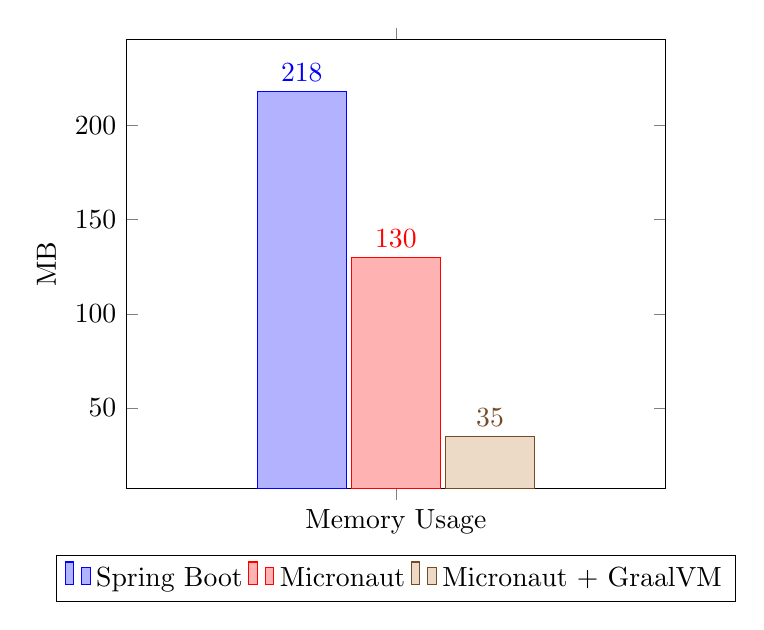
\begin{tikzpicture}
        \begin{axis}[
          ybar,
          bar width=32pt,
          enlargelimits=0.15,
          legend style={at={(0.5,-0.15)},
          anchor=north,legend columns=-1},
          ylabel={MB},
          symbolic x coords={Memory Usage},
          xtick=data,
          nodes near coords,
          nodes near coords align={vertical},
        ]
          \addplot coordinates {(Memory Usage,218)};
          \addplot coordinates {(Memory Usage,130)};
          \addplot coordinates {(Memory Usage,35)};
          \legend{Spring Boot,Micronaut,Micronaut + GraalVM}
        \end{axis}
      \end{tikzpicture}
    \end{center}
  \end{frame}


  \begin{frame}[t]{Time to First Response}
    \begin{center}
      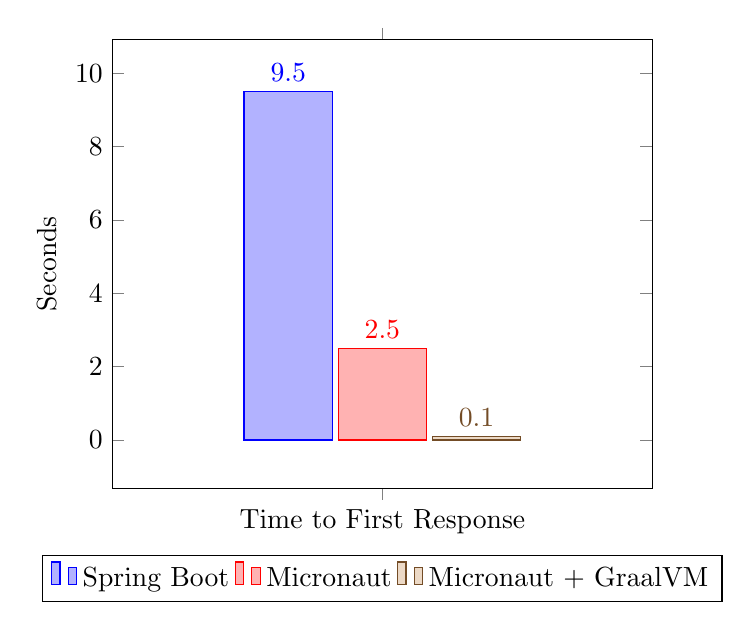
\begin{tikzpicture}
        \begin{axis}[
          ybar,
          bar width=32pt,
          enlargelimits=0.15,
          legend style={at={(0.5,-0.15)},
          anchor=north,legend columns=-1},
          ylabel={Seconds},
          symbolic x coords={Time to First Response},
          xtick=data,
          nodes near coords,
          nodes near coords align={vertical},
        ]
          \addplot coordinates {(Time to First Response, 9.5)};
          \addplot coordinates {(Time to First Response, 2.5)};
          \addplot coordinates {(Time to First Response, 0.1)};
          \legend{Spring Boot,Micronaut,Micronaut + GraalVM}
        \end{axis}
      \end{tikzpicture}
    \end{center}
  \end{frame}

\end{document}
